\documentclass[12pt]{article}
\usepackage{amsmath,amssymb,mathrsfs,fancyhdr,syntonly,lastpage,hyperref,enumitem,graphicx,subcaption, tikz}

\usepackage[thmmarks,thref]{ntheorem}

\theoremstyle{nonumberplain}
\theoremheaderfont{\itshape}
\theorembodyfont{\upshape}
\theoremseparator{.}
\theoremsymbol{\ensuremath{\square}}
\newtheorem{solution}{Solution}

\hypersetup{colorlinks=true,urlcolor=black}

\topmargin      -1.5cm   % read Lamport p.163
\oddsidemargin  -0.04cm  % read Lamport p.163
\evensidemargin -0.04cm  % same as oddsidemargin but for left-hand pages
\textwidth      16.59cm
\textheight     23.94cm
\parskip         7.2pt   % sets spacing between paragraphs
\parindent         0pt   % sets leading space for paragraphs
\pagestyle{empty}        % Uncomment if don't want page numbers
\pagestyle{fancyplain}


\usepackage{Sweave}
\begin{document}
\Sconcordance{concordance:RoughDraft.tex:RoughDraft.Rnw:%
1 25 1 1 0 93 1}

\lhead{\today}
\chead{CSAFE - Hough Grooves Document Process}
\rhead{Page \thepage\ of \pageref{LastPage}}

\section{Introduction}
I do not know how to start introductions!!!!!! 
\section{Methods}


In order to best identify the GEAs we first want to diminish noise in the image. This can be achieved by converting each scan into an image gradient, which signifies where there are directional changes in the color of the image. This approach unforunately loses most of the detail of the three dimensional scans, however, it better highlights the differences between LEAs and GEAs. Once an image gradient is obtained we select only edges we consider to be "strong", meaning they have a magnitude above the 99th percentile. Our reason for not fully carrying out a Canny Edge detection algorithm before using a Hough transform is that the Canny Edge algorithm increases processing time by about 35 seconds per image and actually highlights more striae and breakoff. 

\begin{figure}[!ht]
    \centering
    \begin{subfigure}{.5\textwidth}
      \centering
      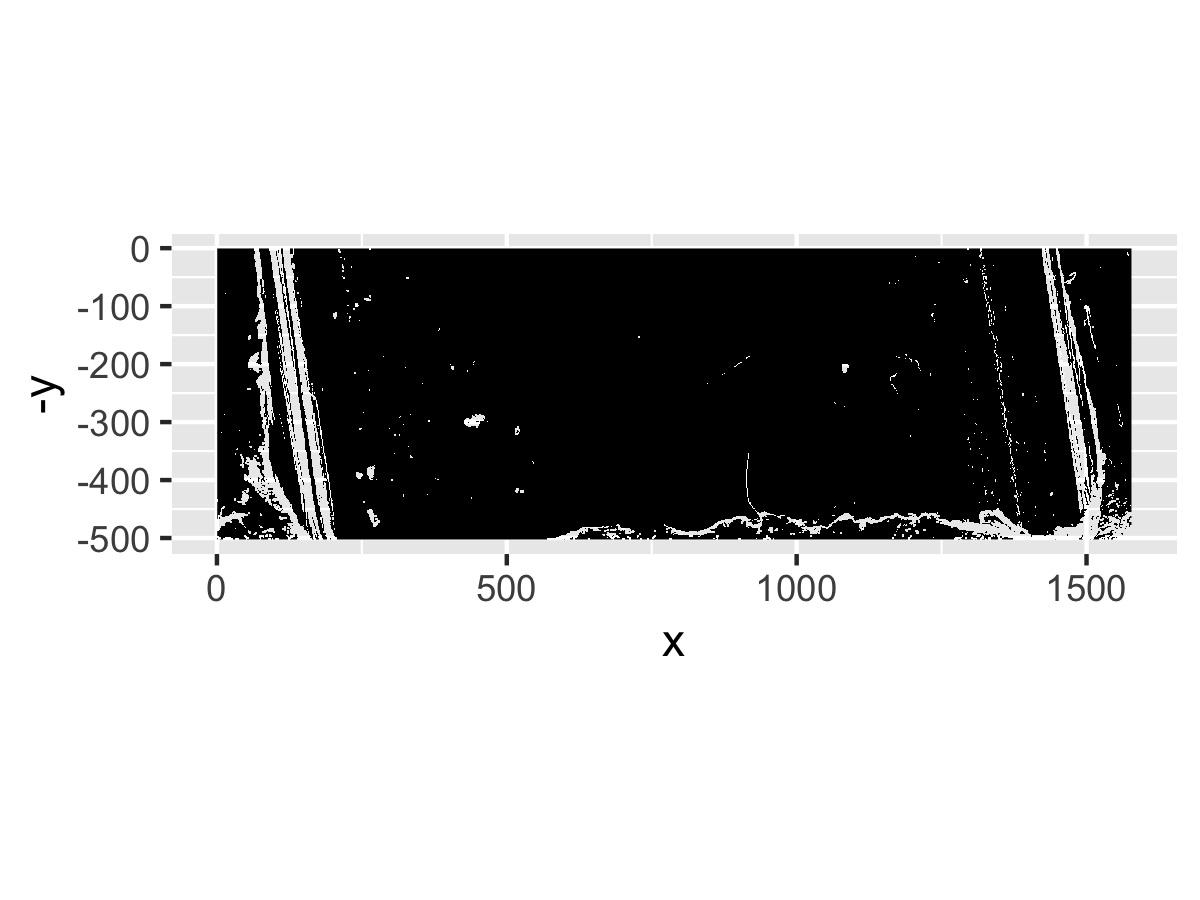
\includegraphics[width = .9\textwidth]{../images/Hamby252_Bullet1_Land3_Strong_edge.png}
      \caption{Edges with magnitudes in the 99th percentile}
      \label{fig: edge1}
      \end{subfigure}%
    \begin{subfigure}{.5\textwidth}
      \centering
      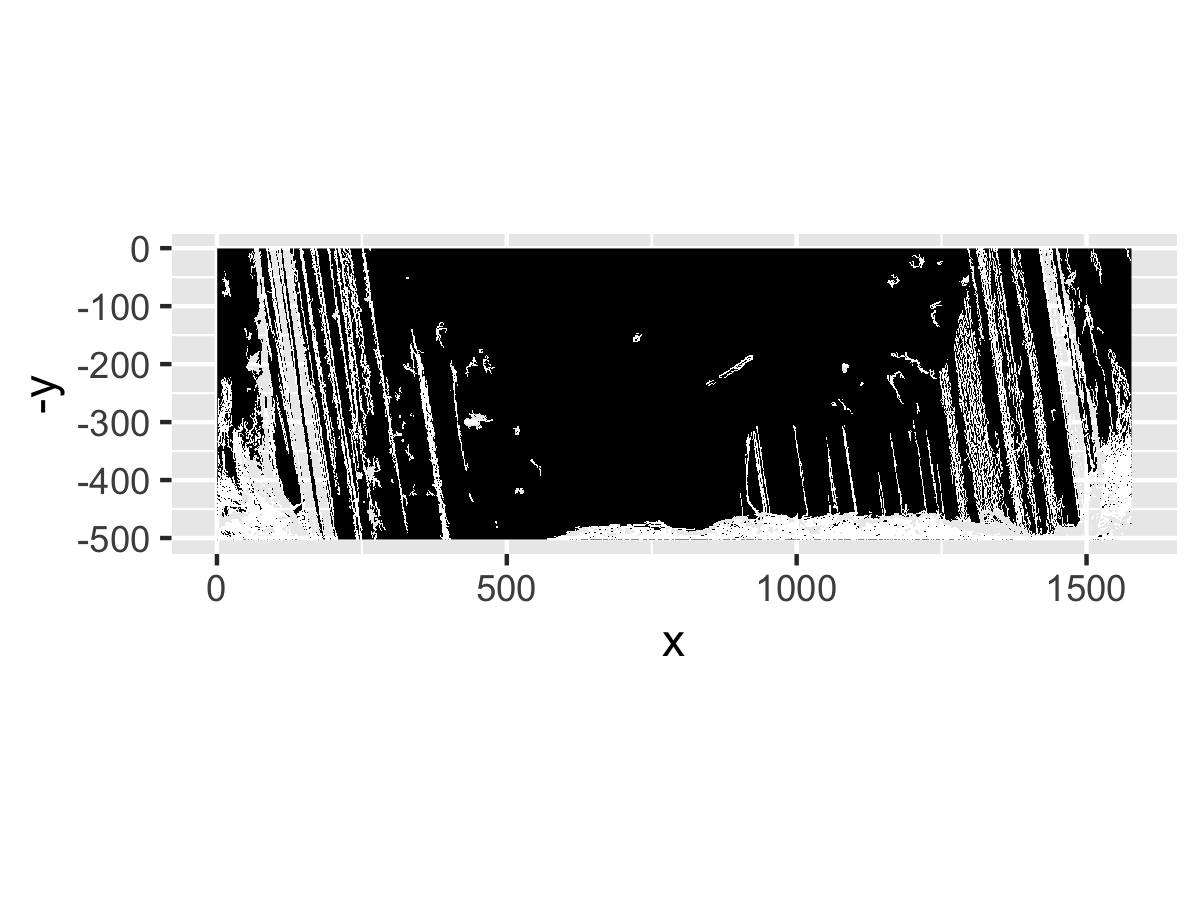
\includegraphics[width = .9\textwidth]{../images/Hamby252_Bullet1_Land3_Canny_Edge.png}
      \caption{Edges improved with Canny edge detection}
      \label{fig: edge2}
      \end{subfigure}
      \caption{Side-by-side comparison of Hamby 252 Bullet using both magnitude thresholding and Canny edge detection}
      \label{fig: canny}
\end{figure}

As shown in Figure \ref{fig: canny} the striae in the LEA are much more pronunced than in the image with only strong edges. We wish to focus on only detecting GEAs, so detecting an increased number of striae through Canny edge detection is not useful for our algorithm. Once we obtain the image gradient with only the strong edges we can then utilize our Hough transformation to obtain generally reasonable estimates of image boundaries. For the Hough transformation we utilize the function `` \texttt{hough\char`_lines}" from the imager package with the number of bins set to 100. While changing the number of bins does not seem to effect the processing time of the Hough transform, having a larger number of bins increases the number of extraneous detected lines in the image. For example in Figure \ref{fig: hough-compare}\subref{fig: hough1} we can see that the Hough transforms with 100 bins does a perfectly aedequate job of picking up the suspected grooves of the bullet. Therefore the extra detected lines in \ref{fig: hough-compare}\subref{fig: hough2} are not used in our analysis so we chose to limit our bin number as a result.

\begin{figure}[!ht]
    \centering
      \begin{subfigure}{.5\textwidth}
      \centering
      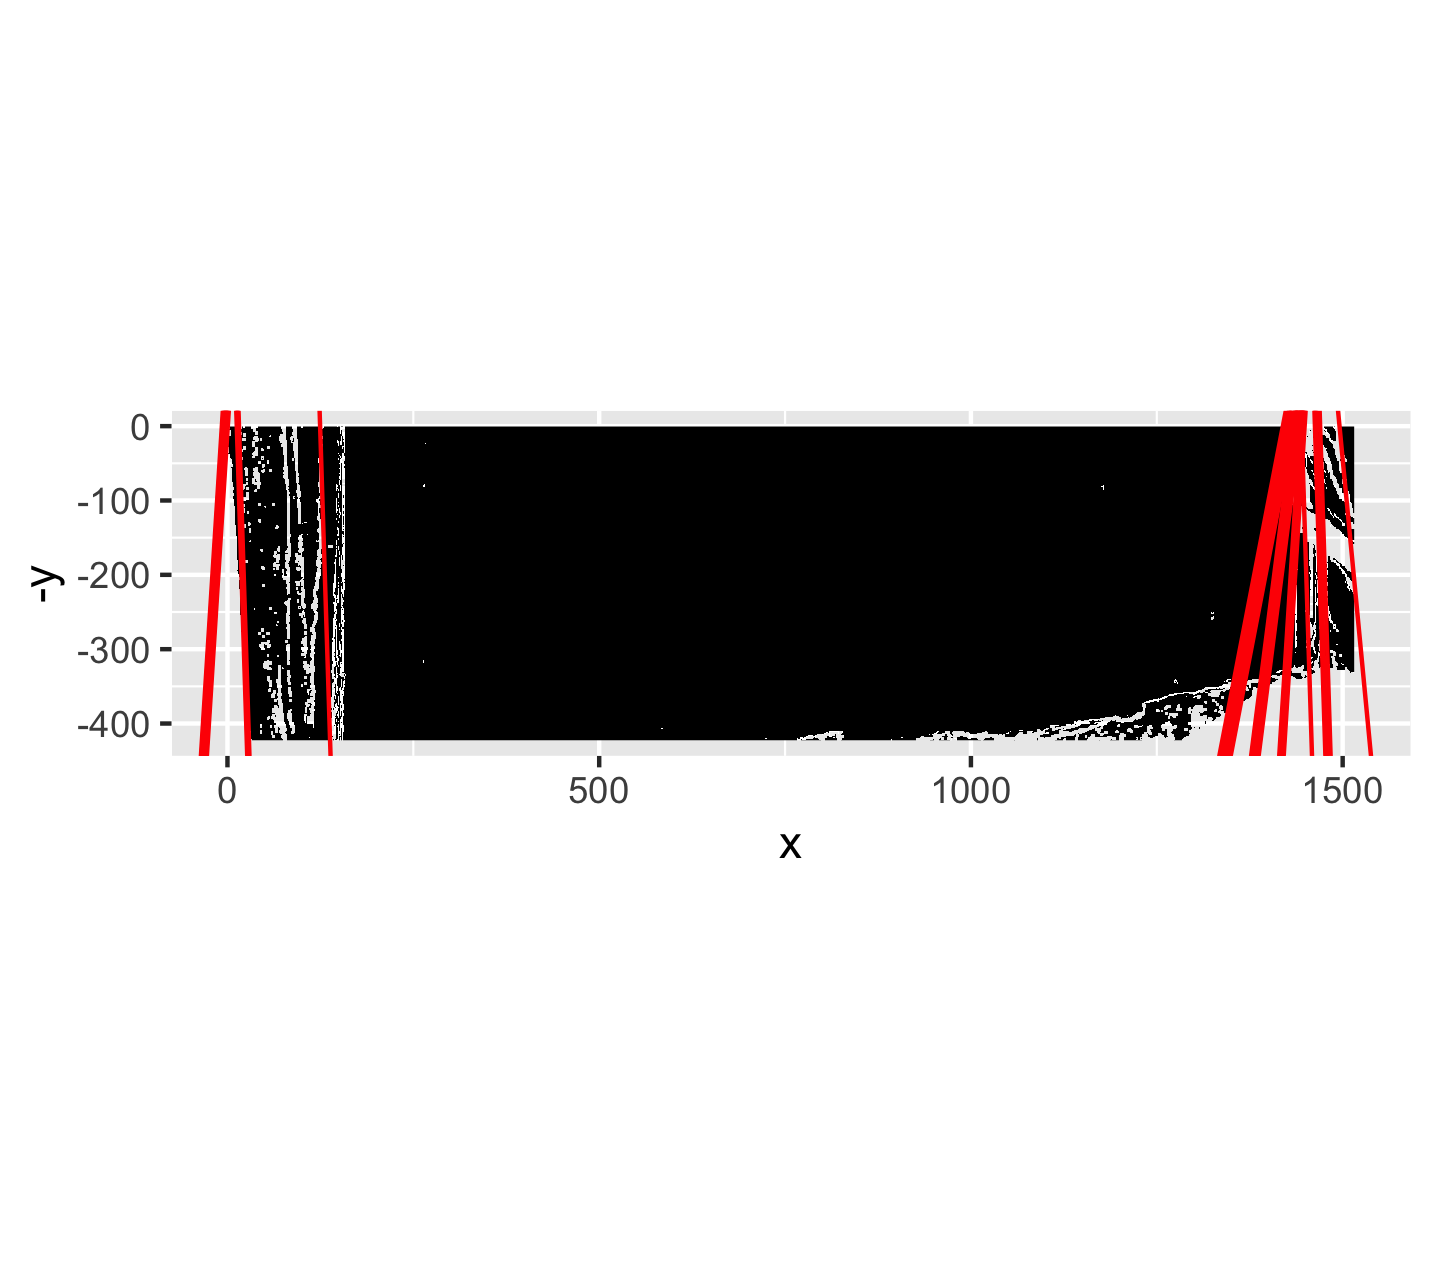
\includegraphics[width = .9\textwidth]{../images/Houston_BarrelF_Bullet1_Hough_Bin100}
      \caption{Hough Transform with 100 bins}
      \label{fig: hough1}
      \end{subfigure}%
    \begin{subfigure}{.5\textwidth}
      \centering
      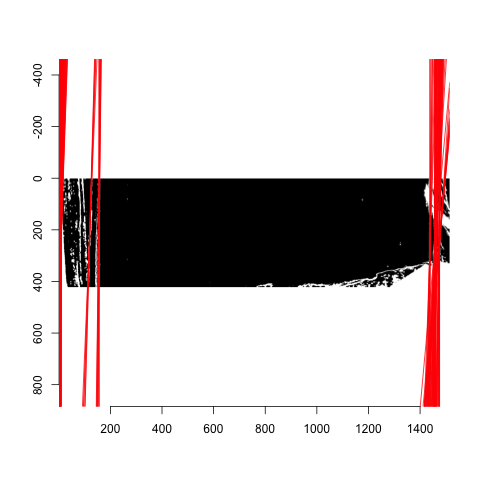
\includegraphics[width = .9\textwidth]{../images/Houston_BarrelF_Bullet1_Hough_Bin900}
      \caption{Hough Transform with 900 bins}
      \label{fig: hough2}
      \end{subfigure}
      \caption{Side-by-side comparison of Houston Barrel F Land 1 Hough Transformation. Hough lines are filtered by having scores in the 99.9th percentile, and having central angles less than $\frac{\pi}{16}$.}
      \label{fig: hough-compare}
\end{figure}

We make the assumption that scans are oriented properly and as such, most Hough lines that correlate to the GEAs will be roughly vertical with some deviations in angle based on scanning technique. It is worth noting that the original output of the `` \texttt{hough\char`_lines}" functions have angles ranging from 0 to $2\pi$. So to make selecting lines from our desired range, easier we chose to transform any angle greater than $\pi$, to instead be from 0 to $-\pi$ by subtracting $2\pi$ from the original theta angle. Therefore we select only the Hough lines that have theta angles from the positive x-axis less than $\frac{\pi}{16}$ and greater than $\frac{-\pi}{16}$. The parametrization produced by `` \texttt{hough\char`_lines}" is of the form:

\begin{center}
$\rho = x \ cos(\theta) \ + \ y \ sin(\theta)$
\end{center}

Where $\rho$ represents the length of the normalized orthogonal vector between the detected line and the origin of the image, and $\theta$ is the angle between the positive x-axis and the normalized vector. We note that the format of bullet images is slightly different from standard x-y-plots. In two-dimensional representations of bullet images, the y-axis is inverted from what we would expect. A reason for this is that the images are processed in \textbf{C++} which stores images, known as ``CImgs'' in a vector format where the first pixel in the vector corresponds to the upper lefthand pixel of the image located at (0,0). Pixels are then ordered from left to right, extending from the origin to the positive x-direction and from top to bottom, from the x-axis towards the negative y-direction. In Figure \ref{fig: parametrization} we see an example of how Hough transforms parametrize a line. In this figure, the orange line represents an example of a detected Hough line. The teal line connecting the origin to the orthogonal bisector of our detected Hough line represents the vector denoted $\rho$ in our above equation. Similarly the teal arc below represents the angle, $\theta$, which is the difference between the top of the image and the orthogonal bisector. 

\begin{figure}[ht!]
  \centering
  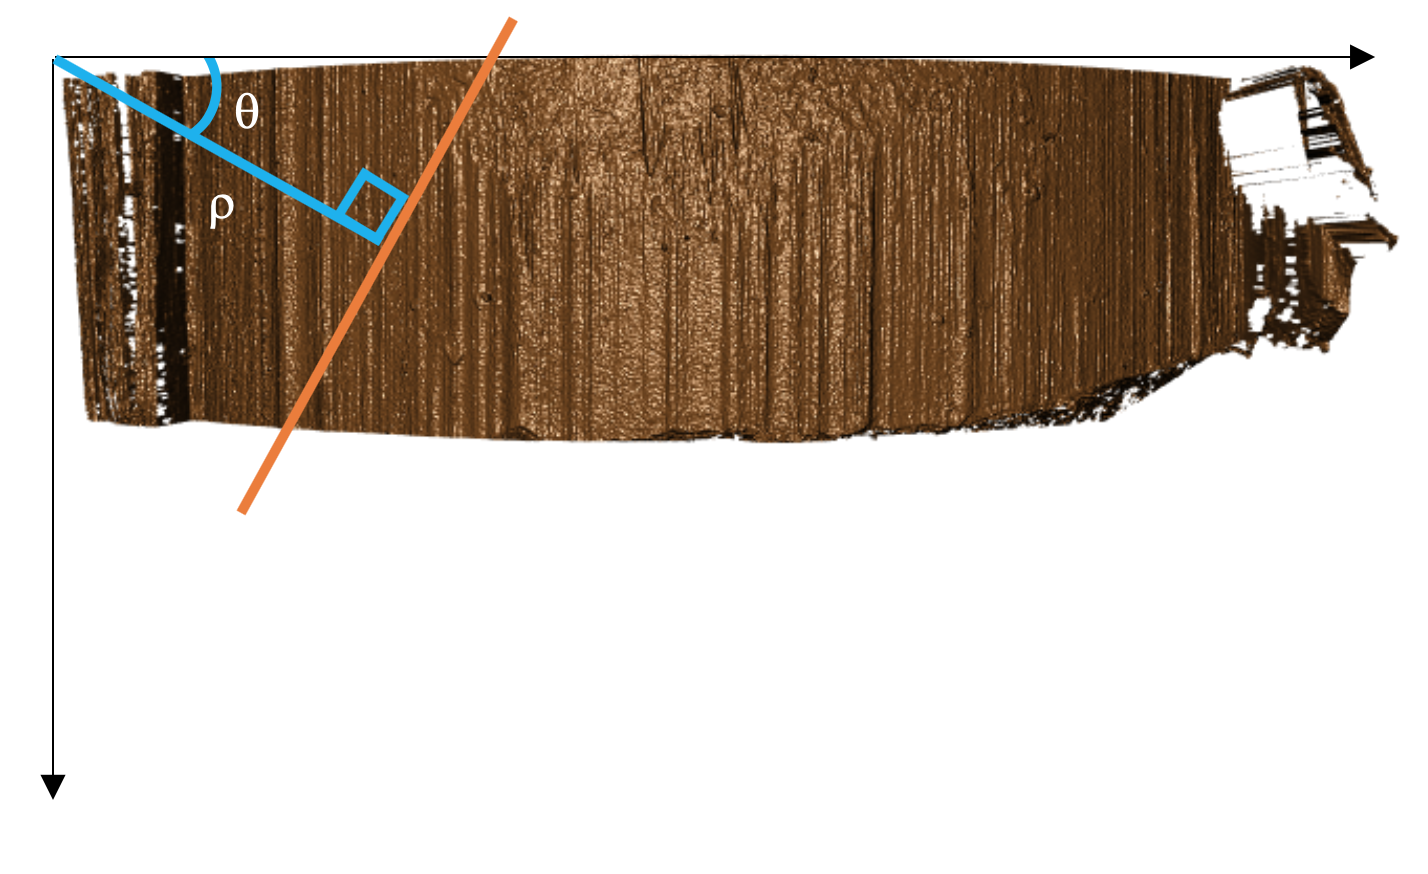
\includegraphics{../images/hessian-example.png}
  \caption{Example of Hessian Normal Form parametrization overlaid a bullet scan}
  \label{fig: parametrization}
\end{figure}

We note that when $\theta$ is equal to 0, the x-intercept is given by $\rho$ however when $\theta$ is not 0 we utilize the above equation to find that the x-intercept is equivalent to $\frac{\rho}{\cos(\theta)}$.  We utilize this calculation to find where the estimated Hough line intersects the top and bottom of the bullet land. The top is the x-intercept calculated previously, however to calculate the bottom intersection of the bullet land we utilize some geometric properties. We can draw a perpendicular line from the x-intercept at the top of the land to the bottom of the land creating a right triangle as shown below in \ref{fig: calcxbottom}. Since both the angle between the orthogonal bisector labeled $\rho$ and the new triangle created from the xintercept to the bottom of the land are both right triangles, we know that the angle at the top of the newly formed triangle is equivalent to $\theta$. Since the x-intercept is known, we can use an elementary geometry technique to calculate the distance labelled $\delta$ in the diagram below. Since $\tan(\theta)$ is equivalent to the proportion of the length of the ``opposite" side over the ``adjacent" side of the right triangle, we know that $\delta = \tan(\theta)*\text{height}$. So the index of the bottom intersection of the bullet land is equivalent to top-intersection - $\delta$. 

\begin{figure}[ht!]
  \centering
  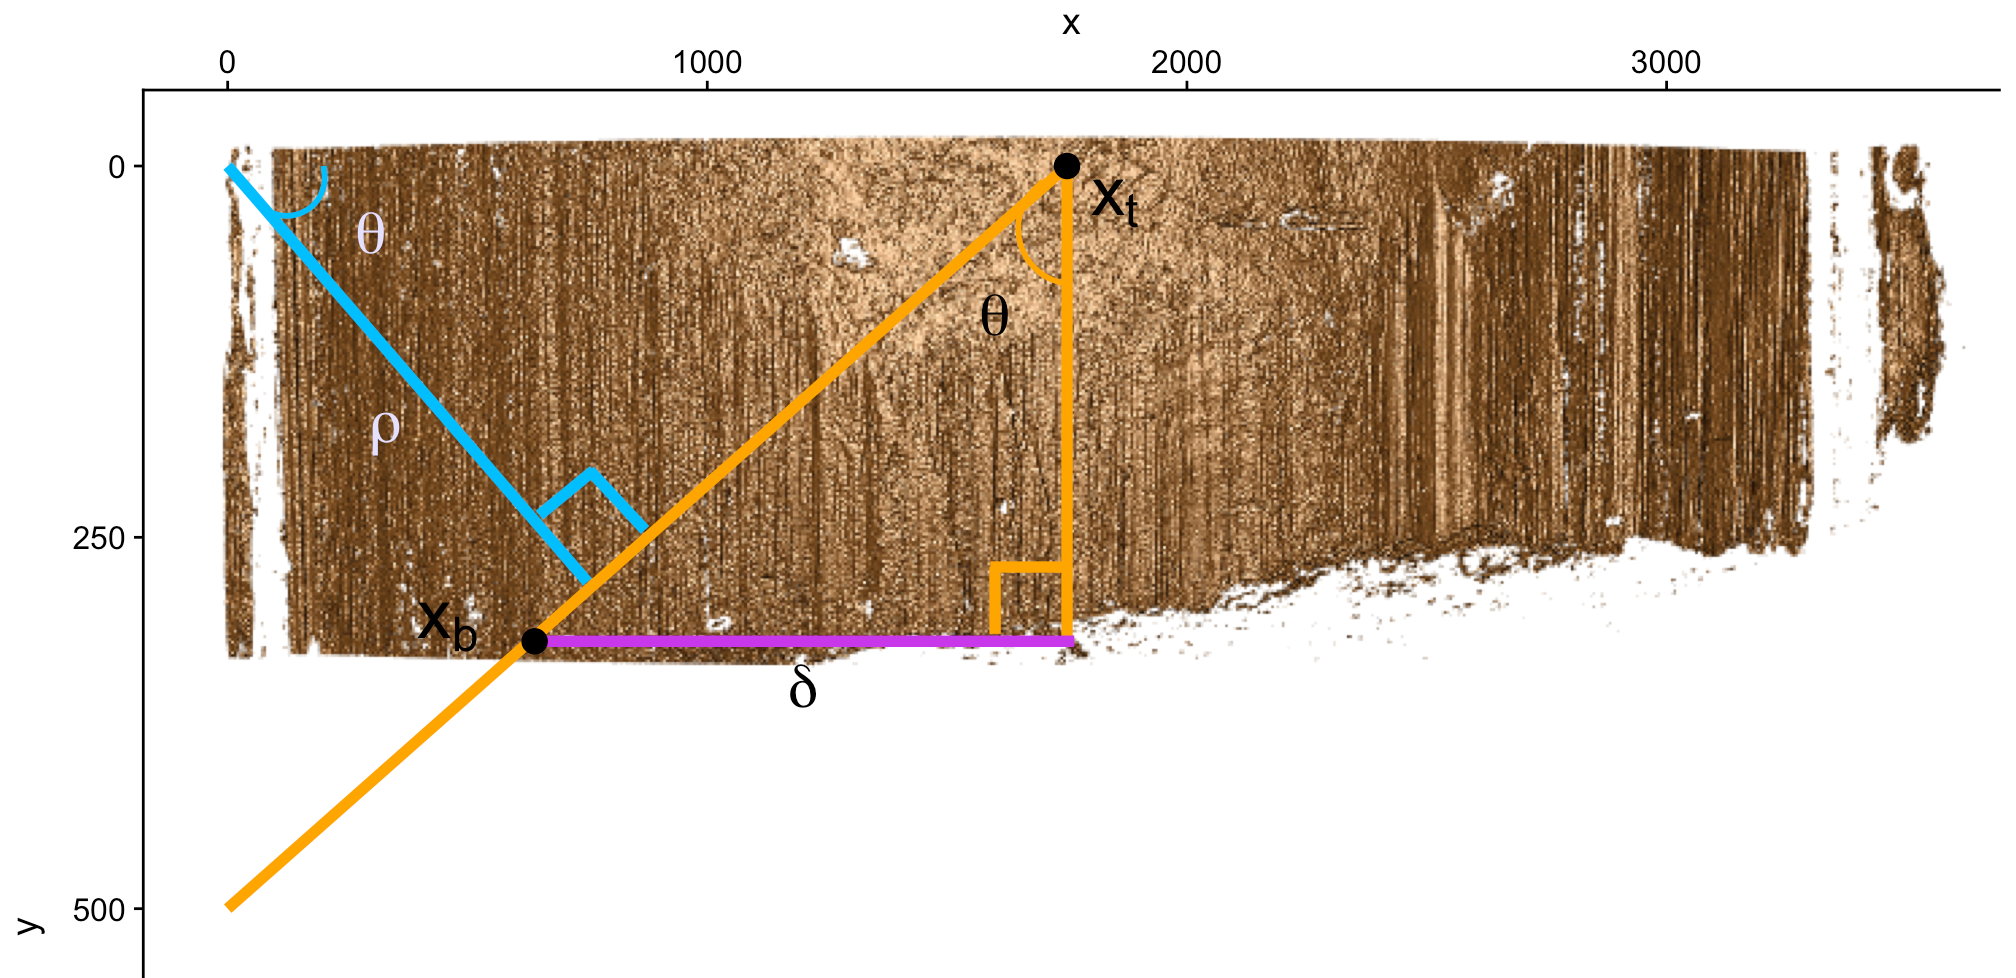
\includegraphics{../images/calc-xbottom.png}
  \caption{Demonstration of calculation of bottom intercept of a bullet land using SOH-CAH-TOA}
  \label{fig: calcxbottom}
\end{figure}

The utility for calculating the top and bottom intercept of our bullet land is that it allows us to calculate the slope of each Hough line with respect to the y-direction. 
\begin{center}
\text{Slope \ with \ respect \ to \ y} = $\frac{(\text{x-intercept of the top} - \text{x-intercept of the bottom})}{\text{height of the bullet land}}$
\end{center}

Traditionally slope in with respect to the x-direction is chosen for describing the equation of a line, however, because we are primarily interested in vertical lines the slope with respect to the x-direction tends to infinity. This is undesireable for a number of reasons, and so we have decided to  

\section{Results?}

In Figure \ref{fig: bestfit1} we show both the middle two thirds of the bullet land and the estimated best fit for the grooves based on our Hough transform. 

\begin{figure}[!ht]
  \centering
  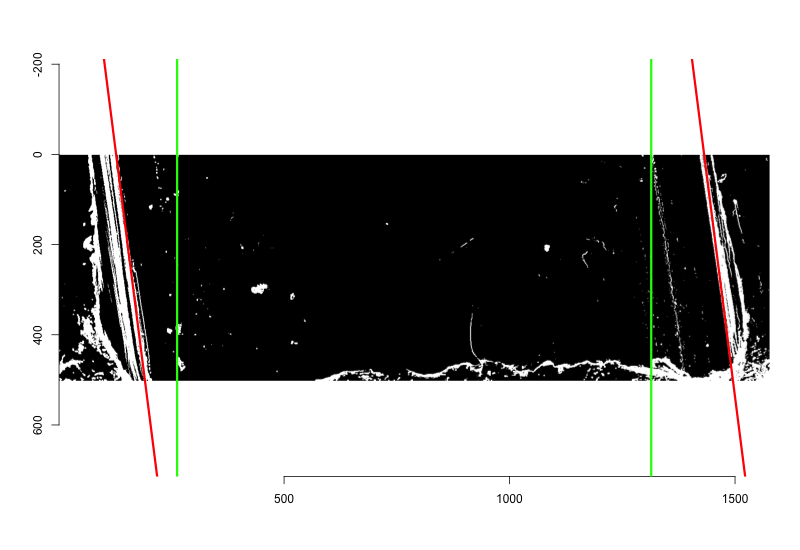
\includegraphics[width = .9\textwidth]{../images/Hamby_252_Bullet1_Land3_BestFit}
  \caption{Houstong Barrel F Bullet 1 middle two-thirds of the bullet land shown in green. Estimated Start of GEA shown in red}
  \label{fig: bestfit1}
\end{figure}
 

\end{document}
